% DO NOT COMPILE THIS FILE DIRECTLY!
% This is included by the the driver file (FlipBeamerTemplate.tex).
\iffalse
{
\setbeamertemplate{footline}{} 
\setbeamertemplate{sidebar right}{\llap{
\includegraphics[width=\paperwidth,height=\paperheight]{BG_upper}}}
\begin{frame}[c]%{\phantom{title page}} 
\phantom{title page}
 \titlepage
\end{frame}
\addtocounter{framenumber}{-1}

}

\fi

\begin{frame}{Teaching Robots How to (Cook/Clean/Fix household items)}

{\bf Q: Can robot learn "how to ..." by themselves}

\begin{itemize}
\item How we learn "how to .." ?
\begin{itemize}
\item Ask experts \quad \emph{Robots asking for help [Tellex et.al.]}
\item Read recipes (recipe books, wikihow.com, e-how.com, etc.) \quad \emph{ Robots making pancake [Beetz et.al.] (single recipe, hard coded perception, hard coded motion)}
\item Watch people performing these tasks (youtube.com, etc.) \quad \emph{activity recognition [Koppula et.al.,  Schiele et.al.]}
\end{itemize}
\end{itemize}
\bf{Large scale, multi-modal, extensive information is available; however, we do not know how to represent/understand them.}	
\end{frame}

\defbeamertemplate{itemize item}{good}{\small
\includegraphics[width=3mm]{good23}}
\defbeamertemplate{itemize item}{bad}{\small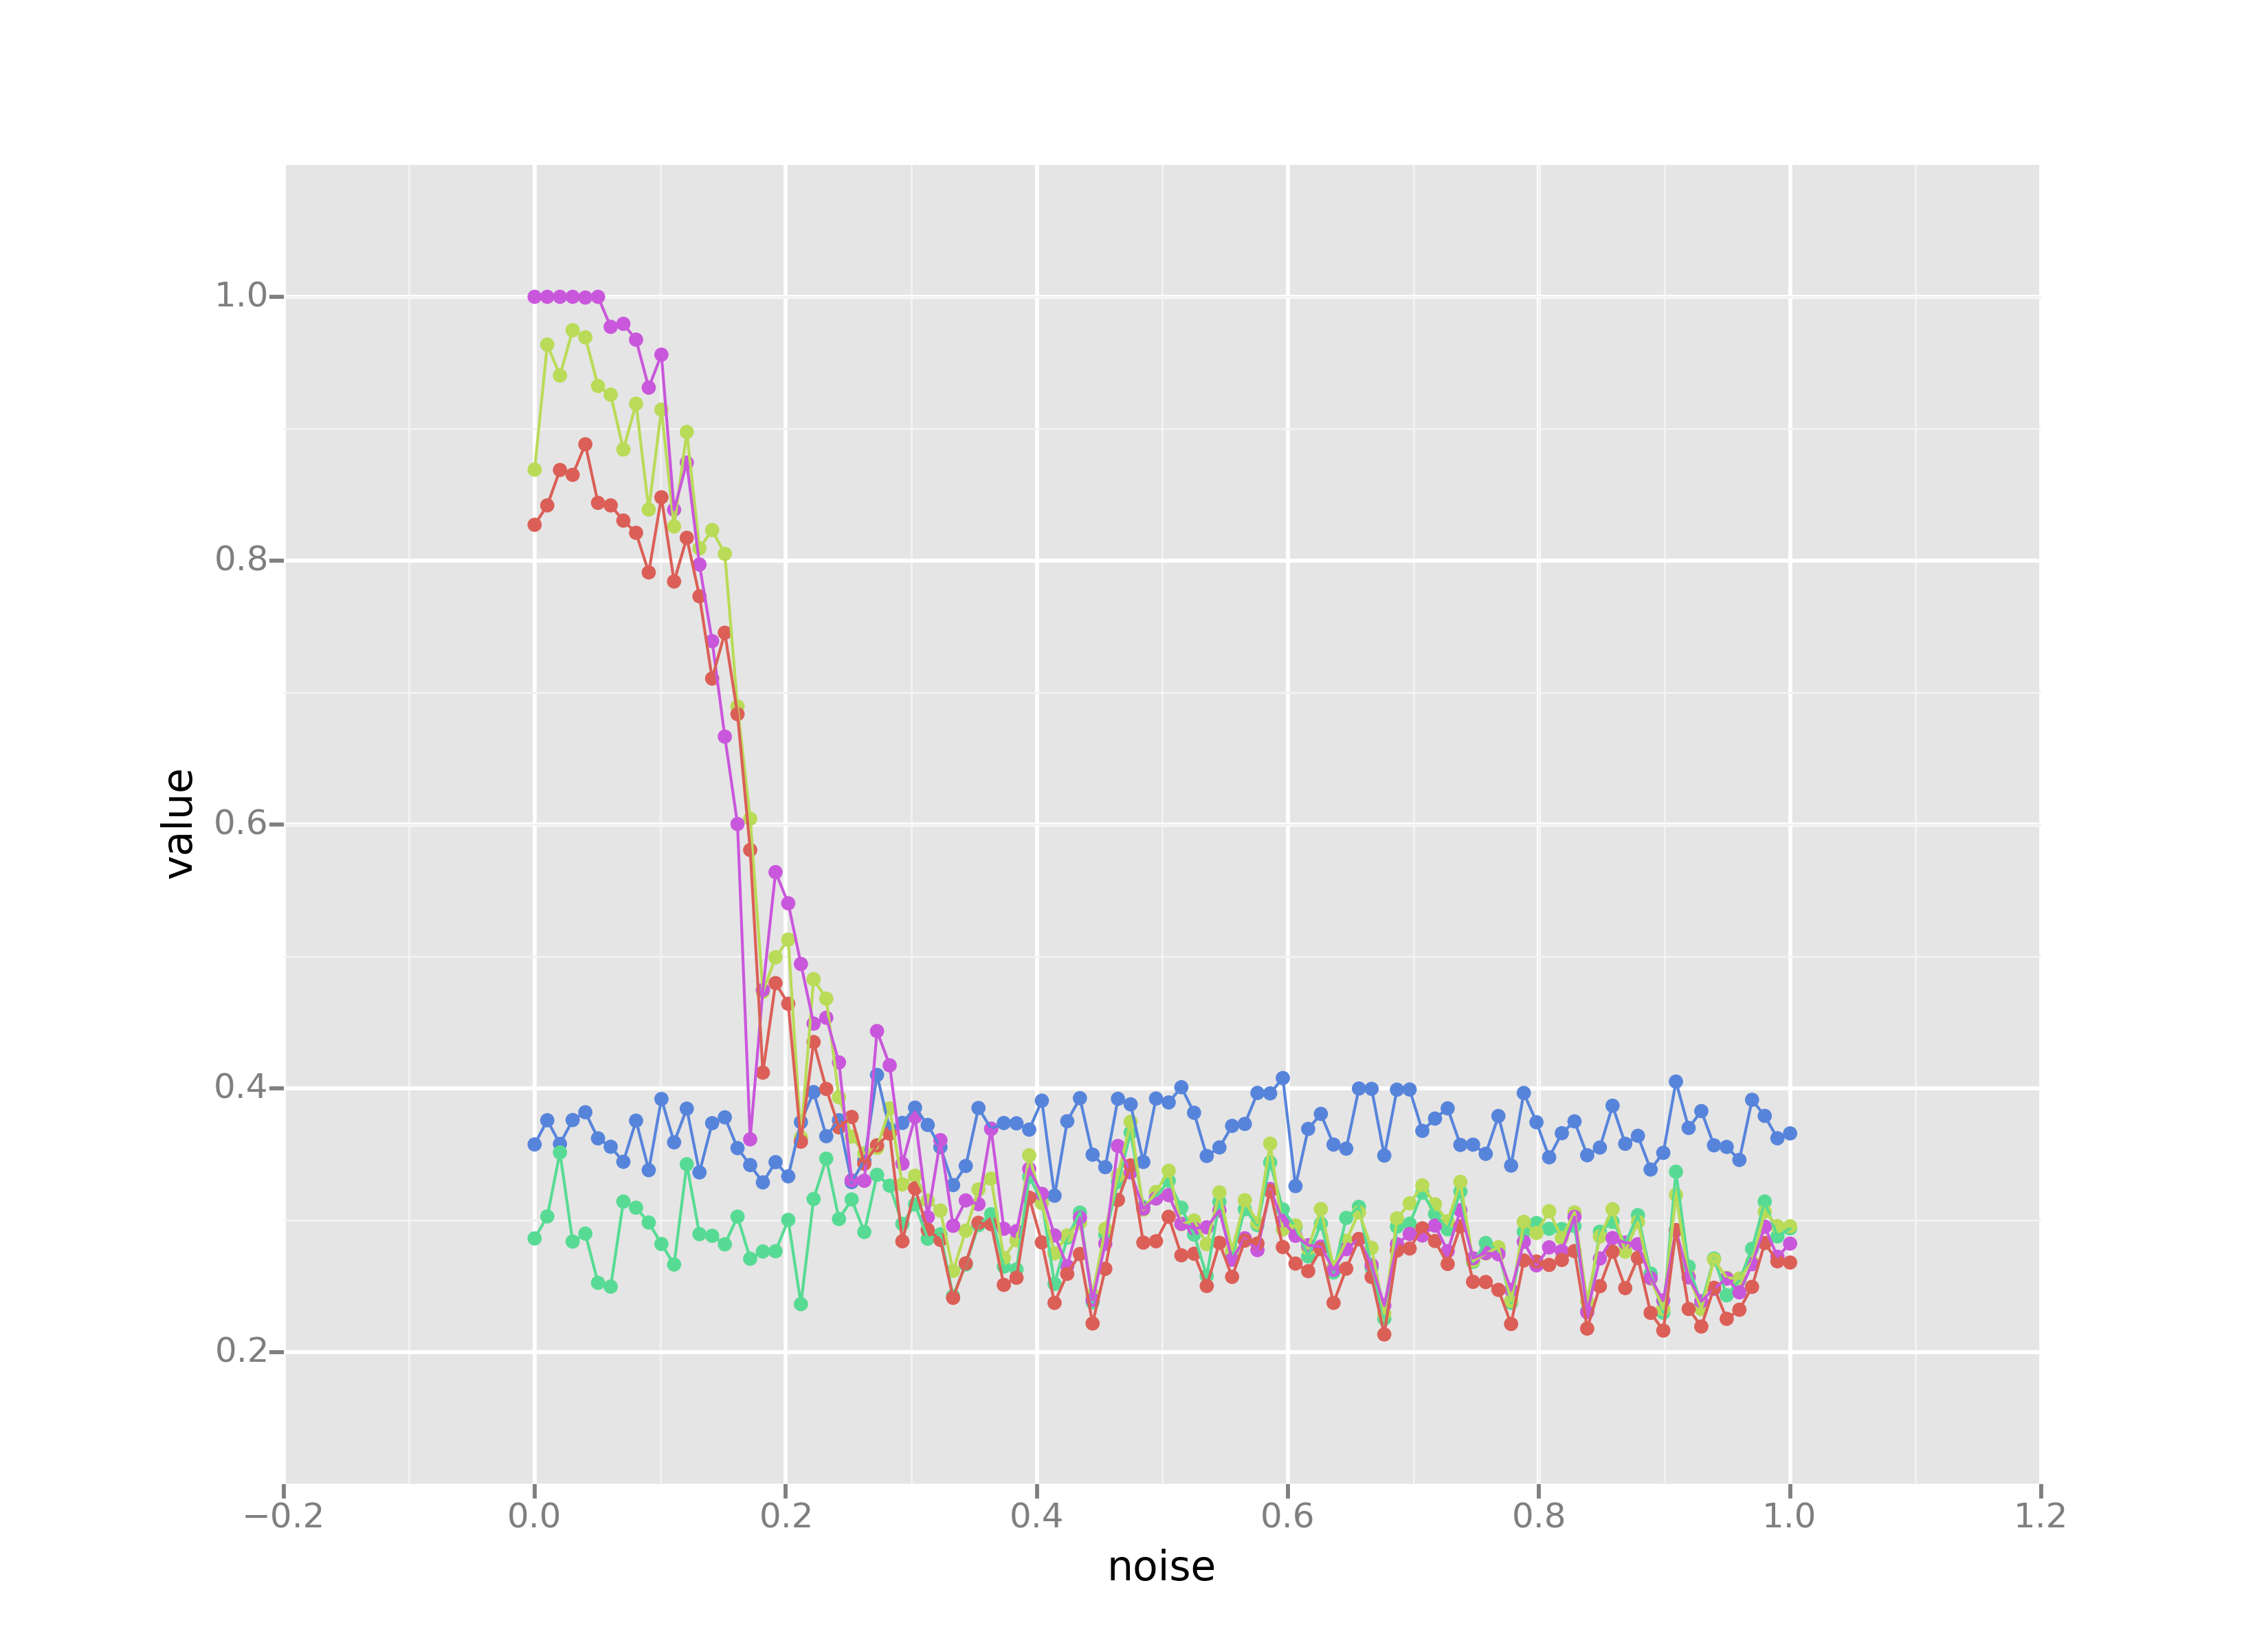
\includegraphics[width=3mm]{error}}

\begin{frame}{Large-Scale Recipes for Daily Activities}{Cooking Recipes, Recipes to fix house hold items/cars}	
\begin{columns}
		\begin{column}[T]{5.5cm}
		{\bf Text Based Resources}\\
		wikihow.com, etc..
		\begin{itemize}
				{\setbeamertemplate{itemize item}[good]
		\item Step-by step natural language description}
						{\setbeamertemplate{itemize item}[bad]
		\item Assume basic human knowledge
		\item Lack specific details (vague descriptions)}
		\end{itemize}
		\end{column}
		\begin{column}[T]{5.5cm}
		{\bf Video Based Resources}\\
		youtube.com, etc..
		\begin{itemize}
		{\setbeamertemplate{itemize item}[good]
		\item Highly detailed and complete information}
								{\setbeamertemplate{itemize item}[bad]
		\item Only a specific example
		\item Lots of environment specific/unrelated information}
		\end{itemize}
		\end{column}
\end{columns}
\vskip1em
						{\setbeamertemplate{itemize item}[bad]
						\begin{itemize}
			\item There are many recipes (both text and video) for a single task -task is ambiguous- (eg 281,000 video, 600 text recipes for \emph{how to tie a bow tie})
			\end{itemize}
			}
\end{frame}

\begin{frame}{Preliminary Set-up}
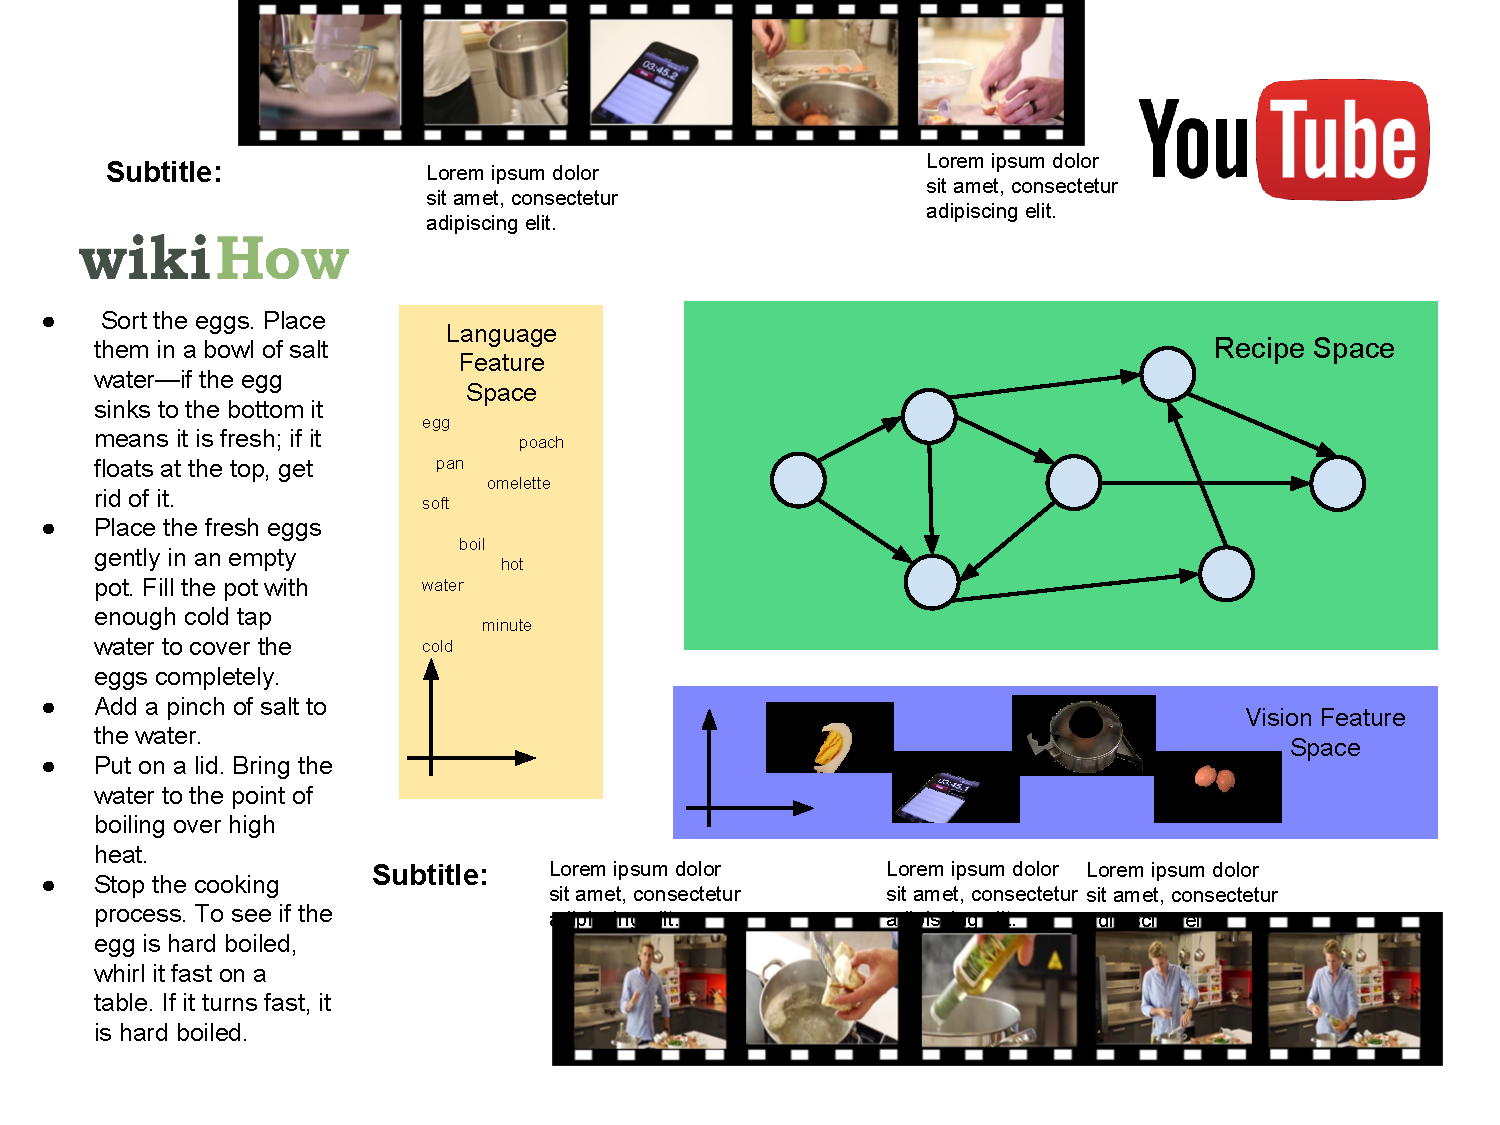
\includegraphics[width=\textwidth]{abc}
\end{frame}


\begin{frame}{Video Object Co-Proposal - Keysegments}
\begin{itemize}
\item Extension of the \emph{Category Independent Object Proposals} to video setting.
\item Basically scoring each region with saliency and motion features. Express similarities as distance of unnormalized histograms. Then, finding the best cluster by using spectral graph clustering. $\max \frac{u^TAu}{u^Tu}$
\item There is no trivial extension to multi-video case
\begin{itemize}
\item If we separately process each video, there are lots of environment specific objects.
\item If we concatenate all object proposals from all videos; there is a serious problem of computational complexity and the result might not be the common object in all videos.
\end{itemize}
\end{itemize}
\end{frame}

\begin{frame}{Multi Video Co-Keysegments}
Solving $\max \sum_{i} \frac{u_i^TA_iu_i}{u_i^Tu_i} + \sum_{i}\sum_{j} \frac{u_i^TA_{ij}u_j}{u_i^T \mathds{1} \mathds{1}^Tu_j}$
\begin{itemize}
\item Tractable if we restrict video relations to k-nn graph.
\end{itemize}
Proposed Algorithm:
\begin{itemize}
\item Crate k-nn graph by using language distance between video descriptions over Youtube.
\item Solve $\max \sum_{i} \frac{u_i^TA_iu_i}{u_i^Tu_i} + \sum_{i}\sum_{j} \frac{u_i^TA_{ij}u_j}{u_i^T \mathds{1} \mathds{1}^Tu_j}$
\end{itemize}

{\bf Intuitive Explanation:} \\
Maximize the normalized cut and average fit within cluster entries

\end{frame}



\begin{frame}{\vspace{-8mm}\\ Solving $\max \sum_{i} \frac{u_i^TA_iu_i}{u_i^Tu_i} + \sum_{i}\sum_{j} \frac{u_i^TA_{ij}u_j}{u_i^T \mathds{1} \mathds{1}^Tu_j}$}

{\bf Good news:}
\begin{itemize}
\item Energy function is quasi-convex.
\item If we fixed the coordinate, it is quasi-linear.
\item It can be optimized by using sub-gradient method.
\end{itemize}

{\bf Gradient is}: \\
\[
\nabla_{u_i} = \frac{2A_i u_i -2u_ir^1(u_i)}{u_i^Tu_i} + \sum_j \frac{1}{u_i^T \mathds{1} \mathds{1}^T u_j} \left( A_{i,j}u_j - u_j^T \mathds{1} r^2(i,j) \right)
\]

\end{frame}



\begin{frame}{Representing Recipes}
Any recipe can be represented as admissible set of sub-tasks, their ordering requirements and their co-occurrence properties.
\end{frame}


\begin{frame}{Observation}
\begin{itemize}
\item Let's denote set of visual objects as $v_0 \ldots v_{M^v}$ and language words as $l_0 \ldots l_{M^l}$.
\item We define Co-Not-Occurrence requirements over a matrices $C^{NO,v}$ and $C^{NO,l}$ as $C^{NO,v}_{i,j} =1$ if $v_i$ and $v_j$ do not occur together. For example, the partial matrix for poaching egg case:
\end{itemize}
\[
 \begin{array}{ccccccc} 
&\rotatebox{90}{Water} & \rotatebox{90}{Pan} & \rotatebox{90}{Tap} & \rotatebox{90}{Gelatin} & \rotatebox{90}{Poacher} & \rotatebox{90}{Cup} \\ 
\text{Water} &  & 0 & 0 & 0 & 0 & 0 \\
\text{Pan} & 0 &  & 0 & 0 & 0 & 0 \\
\text{Tap} & 0 & 0 &  & 0 & 0 & 0 \\
\text{Gelatin} & 0 & 0 & 0 &  & 1 & 1 \\
\text{Poacher} & 0 & 0 & 0 & 1 &  & 1 \\
\text{Cup} & 0 & 0 & 0 & 1 & 1 & 
\end{array} 
\]
\end{frame}

\begin{frame}{Model}
\begin{itemize}
%\item $C^{NO,.}$ is sparse
\item $C^{NO,.}$ is symmetric
%\item If $C^{NO,.}_{i,j}=1$, $C^{No,.}_{i,:}$ is similar to  $C^{No,.}_{j,:}$. Since, they can be replaced.
\item We can relax the ${0,1}$ to $[0,1]$ and obtain the matrix from the observed data.
\end{itemize}
In order to obtain the sub-task co-not-occurrence,
\begin{itemize}
\item Given visual histogram $x^v_0 \ldots x^v_K \in R^{M^v}$ and language histogram $x^l_0 \ldots x^l_K \in R^{M^l}$ of sub-tasks, we can sample co-not-occurrence set $\mathcal{C} \subset [0\ldots K]
 \times [0 \ldots K]$ as;
\begin{itemize}
\item $P((i,j) \in \mathcal{C}) \sim {x^v_i}^T C^{NO,v} x^v_j + {x^l_i}^T C^{NO,l} x^l_j$
\end{itemize} 
\end{itemize}
\end{frame}


\begin{frame}{Model}
Similarly for ordering, we also model it over the extracted visual and language words.
\begin{itemize}
\item We define ordering requirements over a matrices $C^{OR,v}$ and $C^{OR,l}$ as $C^{OR,v}_{i,j} =1$ if $v_i$ has to occur after $v_j$. For example, the partial matrix for poaching egg case:
\end{itemize}
\[
 \begin{array}{ccccccc} 
&\rotatebox{90}{Water} & \rotatebox{90}{Pan} & \rotatebox{90}{Tap} & \rotatebox{90}{Gelatin} & \rotatebox{90}{Poacher} & \rotatebox{90}{Cup} \\ 
\text{Water} &  & 1 & 1 & 0 & 0 & 0 \\
\text{Pan} & 0 &  & 0 & 0 & 0 & 0 \\
\text{Tap} & 0 & 0 &  & 0 & 0 & 0 \\
\text{Gelatin} & 1 & 1 & 1 &  & 0 & 0 \\
\text{Poacher} & 1 & 1 & 1 & 0 &  & 0 \\
\text{Cup} & 0 & 0 & 0 & 0 & 0 & 
\end{array} 
\]
\end{frame}

\begin{frame}{Model}
\begin{itemize}
%\item $C^{OR,.}$ is sparse
\item Either $C^{OR,.}_{i,j}=1$ and $C^{OR,.}_{j,i}=0$ or $C^{OR,.}_{i,j}=0$ and $C^{OR,.}_{j,i}=0$
\item Although it looks quadratic; by keeping an extra observation vector, data can be computed in linear time.
\item We can relax the ${0,1}$ to $[0,1]$ and obtain the matrix from the observed data.
\end{itemize}
In order to obtain the sub-task ordering,
\begin{itemize}
\item Given visual histogram $x^v_0 \ldots x^v_K \in R^{M^v}$ and language histogram $x^l_0 \ldots x^l_K \in R^{M^l}$ of sub-tasks, we can sample ordering set $\mathcal{C} \subset [0\ldots K]
 \times [0 \ldots K]$ as;
\begin{itemize}
\item $P((i,j) \in \mathcal{C}) \sim {x^v_i}^T C^{OR,v} x^v_j + {x^l_i}^T C^{OR,l} x^l_j$
\end{itemize} 
\end{itemize}
\end{frame}


\iffalse 

\begin{frame}{How to Understand Large-Scale Recipes}

{\bf Representation}
\begin{itemize}
\item Represent different recipes of a single task as a structured DAG ?
\item Combine the generality of the text based recipes with the detailed/structured knowledge in videos ?
\end{itemize}
%{\bf Decision}

{\bf Challenges}
\begin{itemize}
\item (Weakly/Un)Supervised learning using large-scale unlabelled/weakly labelled data 
\item Noisy data (unrelated search results etc.)
\item Incomplete data (some recipes will miss some of the steps)
\item Ambiguity of the language
\end{itemize}
%{\bf Decision}
\end{frame}

\begin{frame}{Related Problems}

{\bf Choose the optimal path over the DAG via}
\begin{itemize}
\item (Human User) interactive visualization of the DAG ?
\item (Robot User) environment specifications and hardware limitation (e.g. physical simulation) ?
\end{itemize}
{\bf Nodes with Automatic Tests}
\begin{itemize}
\item Robots/Humans can fail during the execution
\item Can we automatically find a test for each node ?
\item Can we locate the state within the DAG ?
\end{itemize}
\end{frame}

\begin{frame}{Representation Problem}

{\bf Assumptions}
\begin{itemize}
\item Multiple recipes of a single task can be represented as a DAG such that
\begin{itemize}
\item Edges represent actions and nodes represent states with a unique start and end node
\end{itemize}
\end{itemize}

{\bf Representing the Data}
\begin{itemize}
\item Each video represents a path between start and end node (with omitted steps).
\item Each text based recipe represents a set of paths between start node and end node.
\end{itemize}

{\bf Machine Learning Question}
\begin{itemize}
\item Unsupervised multi-modal representation learning to detect activities/objects available in text and video.
\item Given set of incomplete paths between start and end, how can we reconstruct the graph ?
\end{itemize}
\end{frame}

\begin{frame}{Incomplete Review of the Literature}{ Web enabled robots}
\begin{itemize}
\item {\bf Bakebot [Bollini et.al.]:} Manually convert the available recipe to finite state machine and make robot perform it successfully .
\item {\bf Recipe Language Understanding [Beetz et.al., Mori et.al.]:} Converting a specific recipe to a formal plan via language parsing and processing via pre-learned ontologies.
\item {\bf Robots Making Pancake [Beetz et.al.]:} Experimental validation that robots can follow the extracted recipe (no learning). Predefined motion/perception libraries.
\end{itemize}
\end{frame}


\begin{frame}{Incomplete Review of the Literature}{Co-representing text and video}
\begin{itemize}
\item {\bf Text from image [Yang et.al.]:} Text description via object descriptors and a language model.
\item {\bf Grounding action descriptors [Regneri et.al.]} Given videos and text description, find similar action verbs. Later used for paraphrase detection
\item {\bf Domain adaptation [Elhoseiny et.al.]} Given complete text descriptions and incomplete visual information (missing classes), how to train visual classifier. 
\item {\bf Learning visual meanings of text [Zitnick et.al.]:} Given clip-art images and texts, find visual meanings of words like near, run-to, etc.
\end{itemize}
\end{frame}

\begin{frame}{Incomplete Review of the Literature}{Machine learning for graph completion/representation}
\begin{itemize}
\item {\bf Plot Graph [Li et.al.]:} Generate story-graph from crowd source stories. Output is graph represented 
since input is set of nodes.
\item {\bf Network Inference [Nowak et.al., Kubica et.al.]:} An EM algorithm to recover the network topology from the onordered paths. There is no uncertainty about the nodes, only the ordering.
\item {\bf Learning Bayes Networks [Teysier et.al.]:}
\item {\bf StoryLine from Videos and Texts [Gupta et.al.]:} Fully supervised, only and/or graph structure. 
\end{itemize}
\end{frame}
%\item {\bf }\item {\bf }\end{itemize}


\begin{frame}{Datasets/Available Tools}

{\bf Text data:}
\begin{itemize}
\item (Large-scale) Wikihow.com ontology / (Cyc+WordNet)
\item (Large-scale) Some recipe web pages has nice interface/APIs to crawl (cookingforengineers.com)
\end{itemize}

{\bf Visual data:}
\begin{itemize}
\item (Large-scale) some of wikihow.com entries have video/image and they are accessible via API
\item (Large-scale) youtube-dl + youtube search API
\item (Small) CAD-120 dataset of everyday tasks
\end{itemize}

{\bf Text+Visual data:}
\begin{itemize}
\item (Small) Cooking dataset of videos and text descriptions
\item (Small) MSR data of clip-arts representing some daily activities with text descriptions  
\end{itemize}

\end{frame}


\begin{frame}{Preliminary Set-up}

{\bf (Large-scale) wikihow.com/youtube:} After manually choosing a few tasks, crawl wikihow.com recipes and youtube videos.
\begin{itemize}
\item Wikihow crawler is already implemented (there is just one recipe for a single task since this is a wiki)
\item Youtube crawler is already implemented (5k videos per-day limit)
\end{itemize}

{\bf (Small-scale) Basic Indoor Activities:} Enrich the CAD-120 with text based recipes, and use it as an evaluation set-up.

{\bf NLP Tools:} Experimenting with POS tagging/word ontologies to detect synonyms etc. We can use the existing basic setup without changing anything (Stanford CoreNLP, Wordnet, Cyc, Freebase)
\end{frame}



\begin{frame}{Initial Idea}
\begin{itemize}
\item {\bf Object Co-Proposal:} Find the object proposals over the multiple set of videos for the same task.
\item {\bf Dimensionality Reduction:} Represent the small clips by using spatio-temporal relations of the objects. Concatenate with text captions (available for $\sim$ half of the videos - either user provided or ASR).
\item {\bf Subtask proposals:} Cluster the low dimensional visual space+language space.
\item {\bf Generate DAG Graph}
\begin{itemize}
\item {\bf M:} Estimate a CTMC over the set of videos
\item {\bf E:} Compute the probabilities of the videos
\end{itemize}
\end{itemize}
\end{frame}

\begin{frame}{Object Co-Proposal}
Well studied problem in computer vision. Two successful solution directions are:
\begin{itemize}
\item \emph{Category Independent Object Proposals}: Find super-pixels and propose regions. Rank them using a set of features and learning from a dataset (Relatively fast and accurate).
\item \emph{Constrained Parametric Min-Cut/Max-Flow}: Use a pre-learned potential to define Min-Cut/Max-Flow energy function. Generate multiple solutions by varying the parameters (Most accurate solutions, extremely slow).
\end{itemize}
\end{frame}

\begin{frame}{Vidoe Object Co-Proposal - Keysegments}
\begin{itemize}
\item Extension of the \emph{Category Independent Object Proposals} to video setting.
\item Basically scoring each region with saliency and motion features. Express similarities as distance of unnormalized histograms. Then, finding the best cluster by using spectral graph clustering. $\max \frac{u^TAu}{u^Tu}$
\item There is no trivial extension to multi-video case
\begin{itemize}
\item If we separately process each video, there are lots of environment specific objects.
\item If we concatenate all object proposals from all videos; there is a serious problem of computational complexity and the result might not be the common object in all videos.
\end{itemize}
\end{itemize}
\end{frame}

\begin{frame}{Multi Video Co-Keysegments}
Solving $\max \sum_{i} \frac{u_i^TA_iu_i}{u_i^Tu_i} + \sum_{i}\sum_{j} \frac{u_i^TA_{ij}u_j}{u_i^Tu_iu_j^Tu_j}$
\begin{itemize}
\item Still computationally intractable.
\item Solution is keeping video relations to k-nn graph.
\end{itemize}
Proposed Algorithm:
\begin{itemize}
\item Crate k-nn graph by using language distance between video descriptions over Youtube.
\item Solve $u_i^0 = \arg\max \frac{u_i^TA_iu_i}{u_i^Tu_i}$ via power iteration
\item Iteratively solve $\max \sum_{i} \frac{u_i^TA_iu_i}{u_i^Tu_i} + \sum_{i}\sum_{j} \frac{u_i^TA_{ij}u_j}{u_i^Tu_iu_j^Tu_j}$
\end{itemize}
\end{frame}

\begin{frame}{\vspace{-8mm}\\Solving $\max \sum_{i} \frac{u_i^TA_iu_i}{u_i^Tu_i} + \sum_{i}\sum_{j} \frac{u_i^TA_{ij}u_j}{u_i^Tu_iu_j^Tu_j}$}
$r^1(u_i)+r^2(u_i,u_j)=\sum_{i} \frac{u_i^TA_iu_i}{u_i^Tu_i} + \sum_{i}\sum_{j} \frac{u_i^TA_{ij}u_j}{u_i^Tu_iu_j^Tu_j}$
\begin{align*}
&\nabla_{u_i} r^1(u_i)+r^2(u_i,u_j) = \\ &= 2A_i u_i - 2u_i r^1(u_i) + \sum_j \frac{A_{ij}u_j}{u_j^Tu_j} - 2\sum_j u_i r^2(u_i,u_j)
\end{align*}
If we equate to $0$ and write the fixed point iteration,
\begin{equation*}
u_i^{t+1} = \frac{1}{r^1(u_i^t)+r^2(u_i^t,u_j^t)}\left[A_iu_i^t+\frac{1}{2}\sum_j \frac{A_{ij}u_j^t}{u_j^{t^T}u_j^t}\right]
\end{equation*}
\end{frame}


\begin{frame}{Multi Video Co-Keysegments - August 5}
Previous idea failed due to the
\begin{itemize}
\item Dimensionality mismatch.
\item Non-convex energy function.
\end{itemize}
{\bf Solution:} \\
Update the energy function to have dimensionality match  \\

$\max \sum_{i} \frac{u_i^TA_iu_i}{u_i^Tu_i} + \sum_{i}\sum_{j} \frac{u_i^TA_{ij}u_j}{u_i^T \mathds{1} \mathds{1}^Tu_j}$

{\bf Intuitive Explanation:} \\
Maximize the normalized cut and average fit within cluster entries
\end{frame}


\begin{frame}{\vspace{-8mm}\\ Solving $\max \sum_{i} \frac{u_i^TA_iu_i}{u_i^Tu_i} + \sum_{i}\sum_{j} \frac{u_i^TA_{ij}u_j}{u_i^T \mathds{1} \mathds{1}^Tu_j}$}

{\bf Good news:}
\begin{itemize}
\item Energy function is quasi-convex.
\item If we fixed the coordinate, it is quasi-linear.
\item It can be optimized by using sub-gradient method.
\end{itemize}

{\bf Gradient is}: \\
\[
\nabla_{u_i} = \frac{2A_i u_i -2u_ir^1(u_i)}{u_i^Tu_i} + \sum_j \frac{1}{u_i^T \mathds{1} \mathds{1}^T u_j} \left( A_{i,j}u_j - u_j^T \mathds{1} r^2(i,j) \right)
\]

\end{frame}

\begin{frame}{Experiment results for 2 Videos case}

\begin{itemize}
\item Independent Normalized Cut
\item Co-Localization (Keving Tang, Fei-Fei Li)
\item Co-Cluster
\end{itemize}
\end{frame}

\begin{frame}{Next Week(s) Plans}
\begin{itemize}
\item 10 Videos experiment
\item Improve Object Co-Proposal Performance
\begin{itemize}
\item Try different set of region proposals
\item Find the best features (currently it is un-normalized histogram)
\item Optimize parameters
\end{itemize}
\item Represent each frame as histogram of clusters and their motions
\end{itemize}
\end{frame}

\begin{frame}{Time Stamp}
August 26
\end{frame}

\begin{frame}{Recipes to Work On}
\begin{itemize}
\item Hard Boil an Egg‏‎ (Objects are extracted from 10 Videos)
\item Make Scrambled Eggs‏‎ (Pre-processing is done, objects will be extracted)
\item Poach an Egg‏‎ (Pre-processing is done, objects will be extracted)
\end{itemize}
\end{frame}

\begin{frame}{Scaling Issues}
\begin{itemize}
\item Previous Implementation was not scalable
\begin{itemize}
\item Current implementation is fully parallel.
\item It uses L-BFGS to find the the Co-Proposals.
\end{itemize}
\item Improve Object Co-Proposal Performance
\item Try different set of region proposals
\item Find the best features (currently it is un-normalized histogram)
\begin{itemize}
\item Replaced the region proposals with the CPMC(Constrained Parametric Min-Cut)
\item As a feature, two options are implemented Dense Sift and histogram of LAB Color Space.
\end{itemize}
\end{itemize}
10 Videos test results
\end{frame}


\begin{frame}{Representation of the Frame}
\begin{itemize}
\item To represent object proposals, we can use either GMM or mean of the extracted histograms/sifts. In other words, given cluster $i$, we represent it as $\bar{x_i}$.
\item From wikiHow entry, find all salient action verbs, salient object names and their synonyms. 
\item In order to represent each frame, I propose;
\begin{itemize}
\item Propose $M$ object segments from the frame.
\item For each segment, find the nearest cluster(Co-Proposal) and assign to it.
\item Compute the histogram of segments.
\item If subtitle exist, compute the histogram of words.
\item Concatenate two histograms.
\end{itemize}
\end{itemize}
\end{frame}

\begin{frame}{Next Week Plan}
\begin{itemize}
\item Running object proposals on 3 Recipes (10 Videos each).
\item Representing each frame.
\item Running baseline clustering.
\end{itemize}
\end{frame}

\begin{frame}{Time Stamp}
September 2
\end{frame}

\begin{frame}{This Week}
\begin{itemize}
\item (Not Finished) Running object proposals on 3 Recipes (10 Videos each).
\begin{itemize}
\item Data is too noisy, I need to manually discard some videos.
\end{itemize}
\item (Baseline Version) Representing each frame.
\item (Baseline Version) Running baseline clustering.
\end{itemize}
\end{frame}

\begin{frame}{Baseline Clustering}
\begin{itemize}
\item Although the baseline model do not include any temporal reference, resulting clusters are continuous (mostly)
\item Language(Sub-title) information seems noisy, but there is still nice anchor words like drain etc.
\end{itemize}
\end{frame}

\begin{frame}{Problem Definition}
\begin{itemize}
\item Is solving the problem without wikiHow {\bf possible} ?
\item Is solving the problem without wikiHow {\bf more interesting} ?
\end{itemize}
\end{frame}


\begin{frame}{Evaluation}
We need to evaluate;
\begin{itemize}
\item Temporal segmentation
\item Representing video as sequence of sub-tasks
\item Language reference quality.
\end{itemize}

Metric;
\begin{itemize}
\item $\Delta_T=$ IOU metric for temporal segments after labelling.
\item $\Delta_S=$ Smallest string matching distance between ground truth and resulting sequence. 
\item $\Delta_L=$ F-measure between extracted action/object names vs ground truth action object names.
\end{itemize}
\end{frame}

\begin{frame}{Next Week(s) Plan}
\begin{itemize}
\item Running baseline s on 3 Recipes (10 Videos each).
\item Fixing bugs/optimizing parameters and finalizing the baseline.
\item Language Only, Vision Only Tests.		
\item Measuring performance.
\item Labelling videos. 
\end{itemize}
\end{frame}

\begin{frame}{Representing Recipes}
Any recipe can be represented as admissible set of sub-tasks, their ordering requirements and their co-occurrence properties.
\end{frame}

\begin{frame}{Co-occurrence}
 Using co-occurrence has problems like:
\begin{itemize}
\item Co-occurrence is generally modelled to be transitive, but within the recipes they are not. For example, (boiling, using a poacher) and (boiling, using a cup to poach) co-occurs while poaching an egg; but, (using a poacher, using a cup to poach) never occurs.
\item Number of admissible co-occurrence is high; hence, we need more data.
\end{itemize}
Hence, we need to model {\bf co-not-occurrence} for sparsity and intuitive understanding.
\end{frame}

\begin{frame}{Ordering}
Some sub-tasks have ordering requirements like pan need to be filled with water before boiling. Hence, we need to model a set of ordering requirements as well.
\end{frame}

\begin{frame}{Model}
\begin{itemize}
\item Since sub-tasks are latent within the application, we can not model co-not-occurrence and ordering over sub-tasks. 
\item We can model these relations over the atomic concepts which sub-tasks are using. Hence, We model them over extracted visual objects and extracted words.
\end{itemize}
\end{frame}


\begin{frame}{Model}
\begin{itemize}
\item Let's denote set of visual objects as $v_0 \ldots v_{M^v}$ and language words as $l_0 \ldots l_{M^l}$.
\item We define Co-Not-Occurrence requirements over a matrices $C^{NO,v}$ and $C^{NO,l}$ as $C^{NO,v}_{i,j} =1$ if $v_i$ and $v_j$ can not occur together. For example, the partial matrix for poaching egg case:
\end{itemize}
\[
 \begin{array}{ccccccc} 
&\rotatebox{90}{Water} & \rotatebox{90}{Pan} & \rotatebox{90}{Tap} & \rotatebox{90}{Gelatin} & \rotatebox{90}{Poacher} & \rotatebox{90}{Cup} \\ 
\text{Water} &  & 0 & 0 & 0 & 0 & 0 \\
\text{Pan} & 0 &  & 0 & 0 & 0 & 0 \\
\text{Tap} & 0 & 0 &  & 0 & 0 & 0 \\
\text{Gelatin} & 0 & 0 & 0 &  & 1 & 1 \\
\text{Poacher} & 0 & 0 & 0 & 1 &  & 1 \\
\text{Cup} & 0 & 0 & 0 & 1 & 1 & 
\end{array} 
\]
\end{frame}

\begin{frame}{Model}
\begin{itemize}
\item $C^{NO,.}$ is sparse
\item $C^{NO,.}$ is symmetric
\item If $C^{NO,.}_{i,j}=1$, $C^{No,.}_{i,:}$ is similar to  $C^{No,.}_{j,:}$. Since, they can be replaced.
\item We can relax the ${0,1}$ to $[0,1]$ and obtain the matrix from the observed data.
\end{itemize}
In order to obtain the sub-task co-not-occurrence,
\begin{itemize}
\item Given visual histogram $x^v_0 \ldots x^v_K \in R^{M^v}$ and language histogram $x^l_0 \ldots x^l_K \in R^{M^l}$ of sub-tasks, we can sample co-not-occurrence set $\mathcal{C} \subset [0\ldots K]
 \times [0 \ldots K]$ as;
\begin{itemize}
\item $P((i,j) \in \mathcal{C}) \sim {x^v_i}^T C^{NO,v} x^v_j + {x^l_i}^T C^{NO,l} x^l_j$
\end{itemize} 
\end{itemize}
\end{frame}


\begin{frame}{Model}
Similarly for ordering, we also model it over the extracted visual and language words.
\begin{itemize}
\item We define ordering requirements over a matrices $C^{OR,v}$ and $C^{OR,l}$ as $C^{OR,v}_{i,j} =1$ if $v_i$ has to occur after $v_j$. For example, the partial matrix for poaching egg case:
\end{itemize}
\[
 \begin{array}{ccccccc} 
&\rotatebox{90}{Water} & \rotatebox{90}{Pan} & \rotatebox{90}{Tap} & \rotatebox{90}{Gelatin} & \rotatebox{90}{Poacher} & \rotatebox{90}{Cup} \\ 
\text{Water} &  & 1 & 1 & 0 & 0 & 0 \\
\text{Pan} & 0 &  & 0 & 0 & 0 & 0 \\
\text{Tap} & 0 & 0 &  & 0 & 0 & 0 \\
\text{Gelatin} & 1 & 1 & 1 &  & 0 & 0 \\
\text{Poacher} & 1 & 1 & 1 & 0 &  & 0 \\
\text{Cup} & 0 & 0 & 0 & 0 & 0 & 
\end{array} 
\]
\end{frame}

\begin{frame}{Model}
\begin{itemize}
\item $C^{OR,.}$ is sparse
\item Either $C^{OR,.}_{i,j}=1$ and $C^{OR,.}_{j,i}=0$ or $C^{OR,.}_{i,j}=0$ and $C^{OR,.}_{j,i}=0$
\item Although it looks quadratic; by keeping an extra observation vector, data can be computed in linear time.
\item We can relax the ${0,1}$ to $[0,1]$ and obtain the matrix from the observed data.
\end{itemize}
In order to obtain the sub-task ordering,
\begin{itemize}
\item Given visual histogram $x^v_0 \ldots x^v_K \in R^{M^v}$ and language histogram $x^l_0 \ldots x^l_K \in R^{M^l}$ of sub-tasks, we can sample ordering set $\mathcal{C} \subset [0\ldots K]
 \times [0 \ldots K]$ as;
\begin{itemize}
\item $P((i,j) \in \mathcal{C}) \sim {x^v_i}^T C^{OR,v} x^v_j + {x^l_i}^T C^{OR,l} x^l_j$
\end{itemize} 
\end{itemize}
\end{frame}

\begin{frame}{Generative Model}
\begin{itemize}
\item Sample number of sub-activities $K$ from prior.
\item Sample $K$ cluster centers from language words and visual objects spaces.
\item By using clusters, sample co-not occurrence and co-order matrices from $P(P((i,j) \in \mathcal{C})|x^v_i,x^l_i)$
\item By using co-not occurrence and co-order matrices, sample a graph.
\item From a graph, sample a path for the video and sample a sub-graph for WikiHow entry.
\end{itemize}
\end{frame}	

\begin{frame}{Questions to Answer}
\begin{itemize}
\item Optimization functions to find the matrices.
\item Details of the generative model.
\end{itemize}
\end{frame}	

\fi